\documentclass[10pt]{extarticle}
%\documentclass[]{file}
\usepackage[margin=0.2in]{geometry}
\usepackage{romannum}
\usepackage[most]{tcolorbox}
\usepackage{enumitem}
\usepackage{multicol}
\usepackage{hyperref}
\usepackage{eso-pic}
\AddToShipoutPicture*
    {\put(560,750){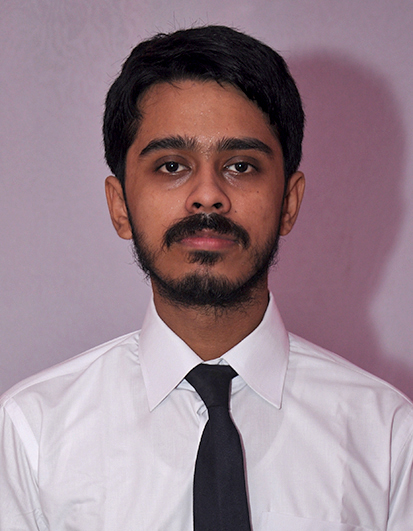
\includegraphics[width=1.2cm,height=1.5cm]{image}}}
\hypersetup{%
  colorlinks=false,% hyperlinks will be coloured
  linkcolor=blue,% hyperlink text will be green
  linkbordercolor=blue,% hyperlink border will be red
}
\setlist[itemize]{noitemsep, topsep=0pt, leftmargin=14pt}
\addtolength{\parskip}{-1.5mm}
\tcbset{
    frame code={}
    center title,
    left=0pt,
    right=0pt,
    top=0pt,
    bottom=0pt,
    colback=gray!50,
    colframe=white,
    width=\dimexpr\textwidth\relax,
    enlarge left by=0mm,
    boxsep=2pt,
    arc=0pt,outer arc=0pt,
    }
\renewcommand{\familydefault}{\sfdefault}
\begin{document}
\begin{flushleft}
\noindent {\huge\textbf{Nirjhar Roy}}
\end{flushleft}
\vspace{-1pt}
\textbf{Email : }babuiroy02@gmail.com, \textbf{Phone : }+91-9038234947

\vspace{-3pt}


%-----------------------------ACADEMICS--------------------------------


\noindent\rule[0.5ex]{\linewidth}{1pt}
{\large \textbf{\begin{tcolorbox}\textsc{\normalsize{Academic Qualifications}}\end{tcolorbox}}}
\vspace{1pt}
\begin{center}
\begin{tabular}{|p{2.5cm}|p{6.0cm}|p{8.5cm}|p{1.8cm}|}
\hline
\centering{\textbf{Year}} & \centering{\textbf{Degree/Certificate}} & \centering{\textbf{Institute}} & \centering{\textbf{CPI/$\%$}}\tabularnewline
\hline
\centering{2018} - Present & \centering{MS(CSE)} & \centering{Indian Institute of Technology, Kanpur(IIT Kanpur)} & \centering{8.00/10}\tabularnewline
\hline
\centering{2012} - {2016} & \centering{B.Tech(CSE)} & \centering{Institute of Engineering and Management, Kolkata(IEM)} & \centering{8.66/10}\tabularnewline
\hline
\centering{2012} & \centering{I.S.C.E(\Romannum{12})} & \centering{Calcutta Boys' School} & \centering{87.6$\%$}\tabularnewline
\hline
\centering{2010} & \centering{I.C.S.E(\Romannum{10})} & \centering{Calcutta Boys' School} & \centering{88.7$\%$}\tabularnewline
\hline
\end{tabular}
\end{center}
\vspace{-1pt}


%-----------------------------WORK EXP--------------------------------

{\large \textbf{\begin{tcolorbox}\textsc{\normalsize{Work Experience}}\end{tcolorbox}}}
\vspace{-2mm}
\begin{itemize}
\item \textbf{Tata Consultancy Services: } I worked as an Assistant Systems Engineer Trainee in a production support team. The project client was \href{https://www.tatacliq.com/}{TATA CLIQ} and my role was to resolve various client and end user issues.
\item \textbf{Duration :} 9 months(25/07/2016 - 09/05/2017)

\end{itemize}
\vspace{-2mm}

%-----------------------------RESEARCH Experience--------------------------------

{\large \textbf{\begin{tcolorbox}\textsc{\normalsize{Research Experience - MS Thesis}}\end{tcolorbox}}}
\vspace{-2mm}
\begin{itemize}
\item \textbf{Securing Demand Paging in Enclave Platforms like \href{https://software.intel.com/en-us/sgx}{Intel SGX} and \href{https://keystone-enclave.org/}{Keystone}} \hfill\hfill(\textit{Jan '19 - Ongoing})\\\textit{Mentor : }\textbf{\href{https://www.cse.iitk.ac.in/users/spramod/}{Dr. Pramod Subramanyan}}, \textit{IIT Kanpur}
\begin{itemize}
    \item \textbf{Aim : }To use some memory access obfuscation algorithms like \href{https://en.wikipedia.org/wiki/Oblivious_RAM}{ORAMs} to prevent information leaks and side channel attacks during demand paging in enclave platforms like Intel SGX and \href{https://keystone-enclave.org/}{Keystone}. We will make our source code open source after our publication.

    \item \textbf{Present Work : }We are using \href{https://keystone-enclave.org/}{Keystone} to implement the page fault handlers and the algorithms. Our algorithm and the page fault handler runs successfully on a real RISCV processor(\href{https://www.sifive.com/boards/hifive-unleashed}{Hifive FU540}) with reasonable performance overheads. Our current progess is:-
      \subitem - Extended keystone runtime to support naive demand paging as well as our secure demand page fault handlers.
      \subitem - Implementation of new attack on a prior work (\href{https://dl.acm.org/doi/10.1145/3307650.3322265}{Invisipage}).
      \subitem - We showed our implementation is more secure than \href{https://dl.acm.org/doi/10.1145/3307650.3322265}{Invisipage} with better performance.
      \subitem - A detailed performance comparison of various oblivious demand paging algorithms(\href{https://en.wikipedia.org/wiki/Oblivious_RAM}{ORAMs}).





\end{itemize}

\end{itemize}
\vspace{-4mm}





%-----------------------------Key Projects--------------------------------


\medskip
{\large \textbf{\begin{tcolorbox}\textsc{\normalsize{Key Projects}}\end{tcolorbox}}}
\vspace{-2mm}
\begin{itemize}

                      %-------------Encrypted Dropbox--------------


\item \textbf{``\href{https://github.com/NirjharRoy/Secure-Dropbox-Testbed-using-GOLANG}{Encrypted Dropbox}" : A cryptographically authenticated and secure file store}\hfill\hfill(\textit{Jan '19 - Apr '19})\\{\textit{Mentor : }}\textbf{\href{https://www.cse.iitk.ac.in/users/spramod/}{Dr. Pramod Subramanyan}}, \textit{{Course : }}\textbf{Computer System Security}, \textit{IIT Kanpur}
\begin{itemize}

\item Designed a file storing and sharing system testbed where the contents are encrypted, and file operation primitives are all secure even if the server is malicious. It won't be able to read or tamper file contents and also to map file contents to its owners.

\end{itemize}


                        %-------------Capture the Flag--------------

\item \textbf{``Capture the Flag" : Binary and Web based attacks attacks}\hfill\hfill(\textit{Jan '19 - Apr '19})\\{\textit{Mentor : }}\textbf{\href{https://www.cse.iitk.ac.in/users/spramod/}{Dr. Pramod Subramanyan}}, \textit{{Course : }}\textbf{Computer System Security}, \textit{IIT Kanpur}
\begin{itemize}
\item Implemented attacks in Binary CTF using Buffer overflow, Integer overflow and web based attacks like Cross-site scripting, CSRF.


\end{itemize}

                        %-------------Trace sim--------------


\item \textbf{Trace Simulator}\hfill\hfill(\textit{May '19 - Dec '19})\\{\textit{Mentor : }}\textbf{\href{https://www.cse.iitk.ac.in/users/spramod/}{Dr. Pramod Subramanyan}}, \textit{IIT Kanpur}
\begin{itemize}
\item Parsing memory access sequence trace of an application and apply various page replacement policies and memory obfuscation algorithms like \href{https://en.wikipedia.org/wiki/Oblivious_RAM}{ORAMs}. This greatly helps in the  study of page replacement policies and other statistics of an application execution.
\end{itemize}





                        %-------------CRAFTML--------------



\item \textbf{ \href{https://github.com/NirjharRoy/CRAFTML}{Implementation of CRAFTML}, an Efficient Clustering based Random Forest for Extreme Multi-label Learning} \\
{\textit{Mentor : }}\textbf{\href{https://www.cse.iitk.ac.in/users/piyush/}{Dr. Piyush Rai}}, \textit{{Course : }}\textbf{Introduction to Machine Learning}, \textit{IIT Kanpur}\hfill\hfill(\textit{Aug '18 - Nov '18})
\begin{itemize}
\item Implemented CRAFTML algorithm with python and tested on datasets like \href{http://manikvarma.org/downloads/XC/XMLRepository.html}{Mediamill, Bibtex, Delicious and Amazon 670K}.

\end{itemize}


%Implemented CRAFTML algorithm and tested on medium scale datasets like \href{http://manikvarma.org/downloads/XC/XMLRepository.html}{Mediamill, Bibtex, Delicious and Amazon 670K}.


                          %-------------Compact Distributed Objects--------------


\item \textbf{Compact Distributed Objects}\hfill\hfill(\textit{Aug '18 - Nov '18})\\{\textit{Mentor : }}\textbf{{Dr. Ratan K. Ghosh}}, \textit{{Course : }}\textbf{Topics in Distributed System}, \textit{IIT Kanpur}
\begin{itemize}
\item A student management system implementation with distributed and compact objects(using \href{https://developers.google.com/protocol-buffers}{Protobuf}) which involved accepting requests from multiple clients and detecting and resolving multi-client request conflicts efficiently. Java was used as the programming language.
\end{itemize}





                %-------------Home automation--------------


\item \textbf{Home Automation and Alert System}\hfill\hfill(\textit{Jan '16 - April '16})\\{\textit{Mentor : }}\textbf{{Prof. Eekian Wong}}, \textit{{Course : }}\textbf{Design Lab}, \textit{Institute of Engineering and Management, Kolkata}
\begin{itemize}
\item Designing an home alert and automated control system for old and physically challenged people, implemented using \href{https://www.arduino.cc/en/Guide/ArduinoUno}{Arduino Uno}.
\end{itemize}



                %-------------Flight management--------------


\item \textbf{Flight Management System}\hfill\hfill(\textit{Jul '14 - Dec '14})\\{\textit{Mentor : }}\textbf{{Prof. Eekian Wong}}, \textit{{Course : }}\textbf{Object Oriented Programming in Java}, \textit{Institute of Engineering and Management, Kolkata}
\begin{itemize}
\item With the primary aim to learn the basic principles of Object oriented programming, we designed a simple flight management system that will give a set of direct flights as well connecting flights with the results being sorted in increasing order of flight duration.
\end{itemize}






%-----------------------------Technical Skills--------------------------------



\end{itemize}
\vspace{-2mm}

{\large \textbf{\begin{tcolorbox}\textsc{\normalsize{Technical Skills}}\end{tcolorbox}}}
\vspace{-2mm}
\begin{itemize}
\itemsep0em
\item \textbf{Programming Languages : }C, C++, Java, Python
\item \textbf{Software and Libraries : } \href{https://www.gnu.org/software/gdb/}{GDB}, Numpy, \href{http://www.gem5.org/}{Gem5}
\end{itemize}

\vspace{-2mm}



%-----------------------------ACHIVEMENTS--------------------------------

{\large \textbf{\begin{tcolorbox}\textsc{\normalsize{Scholastic Achievements}}\end{tcolorbox}}}
\vspace{-2mm}
\begin{itemize}

\item Secured \textbf{All India Rank 377} in \textbf{GATE 2018} amongst 1.1 Lakh candidates with \textbf{99.65} percentile.

\item Secured \textbf{Rank 2505} in \textbf{WBJEE 2012} amongst 1 Lakh candidates with \textbf{97.49} percentile.


\item \textbf{Competitive Coding :} Finalist in FantaC conducted   in B.P. Poddar Institute of Technology,Kolkata in 2015.

\item \textbf{Code Debugging: } \textbf{Finalist in Bugsmash} in I.E.M, Kolkata  in 2015.

\item \textbf{Medals: }Won medals and certificates in school for \textbf{getting above 90\%} in I.C.S.E(best of 5 subjects) and I.S.C.E (best of 4 subjects).



\end{itemize}
\vspace{-2mm}










%-----------------------------Relevant Courses--------------------------------

{\large \textbf{\begin{tcolorbox}\textsc{\normalsize{Relevant Courses}}\end{tcolorbox}}}
\begin{center}
\vspace{-1mm}
\begin{itemize}
\itemsep0em
\item Introduction to Machine Learning, Computer Systems Security, Basic Computer Architecture, Basic Operating Systems, Basic Computer Networks
\end{itemize}
\vspace{-1mm}

\end{center}


\end{document}
